\documentclass[11pt]{article}

\usepackage[margin=1in]{geometry}
\usepackage{hyperref}
\usepackage{enumitem}
\usepackage{parskip}
\usepackage{graphicx}

% Diagram support (portable)
\usepackage{tikz}
\usetikzlibrary{positioning,shapes.geometric}

\title{Incidental Requirements --- Timeline Feature (Ravon Henson)}
\date{}

\begin{document}
\maketitle

\section{Scope}
This document captures functional and non-functional requirements for the \textbf{Timeline} component of \textit{Incidental}, a real-time incident reporting and management system.

\section{Fully Dressed Use Cases (Timeline)}

% ---------- UC-TL-1 ----------
\subsection*{Use Case UC-TL-1: Record System-Generated Timeline Event}
\textbf{Primary Actor:} System (Incidental) \\
\textbf{Supporting Actors:} Integrations/Monitoring (optional), Active users (viewers)

\textbf{Stakeholders and Interests}
\begin{itemize}[nosep]
  \item \textbf{Responders:} want an accurate, chronological history of what happened.
  \item \textbf{Managers:} want an auditable timeline for review and accountability.
  \item \textbf{Stakeholders:} want trustworthy incident progress information.
\end{itemize}

\textbf{Preconditions}
\begin{itemize}[nosep]
  \item An incident exists and is active.
\end{itemize}

\textbf{Success Guarantee (Postconditions)}
\begin{itemize}[nosep]
  \item A new timeline entry is stored with a server-generated timestamp.
  \item Timeline order remains strictly chronological (no manual reordering).
\end{itemize}

\textbf{Main Success Scenario}
\begin{enumerate}[nosep]
  \item A system event occurs (e.g., incident declared, responder assigned, status updated).
  \item The system creates a timeline entry describing the event.
  \item The system assigns a server-generated timestamp to the entry.
  \item The system stores the entry and appends it to the incident timeline.
  \item The system displays the updated timeline to active users.
\end{enumerate}

\textbf{Extensions}
\begin{itemize}[nosep]
  \item \textbf{2a. High-frequency events occur simultaneously}
    \begin{enumerate}[nosep]
      \item The system uses a single authoritative timestamp source.
      \item The system orders events by timestamp (and a stable tie-breaker when needed).
    \end{enumerate}

  \item \textbf{4a. Storage failure}
    \begin{enumerate}[nosep]
      \item The system signals an error and retries persistence.
      \item If retries fail, the system flags timeline persistence as degraded and alerts authorized users.
    \end{enumerate}
\end{itemize}

\textbf{Special Requirements}
\begin{itemize}[nosep]
  \item Users cannot manually reorder entries.
\end{itemize}

\textbf{Technology and Data Variations}
\begin{itemize}[nosep]
  \item Events may originate from user actions, integrations, or internal services.
\end{itemize}

\textbf{Frequency of Occurrence:} High during active incidents.

% ---------- UC-TL-2 ----------
\subsection*{Use Case UC-TL-2: Add Manual Timeline Entry}
\textbf{Primary Actor:} Authorized User (Responder/Engineer) \\
\textbf{Supporting Actors:} System

\textbf{Stakeholders and Interests}
\begin{itemize}[nosep]
  \item \textbf{Responders:} want to record actions taken, observations, and decisions for coordination.
  \item \textbf{Postmortem Owner:} wants complete records for later reporting.
\end{itemize}

\textbf{Preconditions}
\begin{itemize}[nosep]
  \item An incident exists.
  \item User is authorized to add timeline entries.
\end{itemize}

\textbf{Success Guarantee (Postconditions)}
\begin{itemize}[nosep]
  \item The entry is stored and visible in the timeline.
  \item The entry has a server-generated timestamp.
\end{itemize}

\textbf{Main Success Scenario}
\begin{enumerate}[nosep]
  \item User opens the incident timeline.
  \item User selects ``Add Timeline Entry.''
  \item System prompts for entry details (event type and description).
  \item User enters description and selects an event type (e.g., decision, mitigation, responder action, system event).
  \item System assigns a server-generated timestamp.
  \item System stores the entry and displays it in chronological order.
\end{enumerate}

\textbf{Extensions}
\begin{itemize}[nosep]
  \item \textbf{4a. Missing required fields}
    \begin{enumerate}[nosep]
      \item System prompts user to complete missing information.
      \item User revises and resubmits.
    \end{enumerate}

  \item \textbf{2a/4b. User not authorized}
    \begin{enumerate}[nosep]
      \item System rejects the request and displays an authorization error.
    \end{enumerate}
\end{itemize}

\textbf{Special Requirements}
\begin{itemize}[nosep]
  \item Users cannot set or edit timestamps.
  \item Users cannot reorder entries.
\end{itemize}

\textbf{Technology and Data Variations}
\begin{itemize}[nosep]
  \item Event type values may be selected from a predefined list (e.g., decision, mitigation, responder action, system event).
\end{itemize}

\textbf{Frequency of Occurrence:} High during active incidents.

% ---------- UC-TL-3 ----------
\subsection*{Use Case UC-TL-3: Edit Timeline Entry with Revision History}
\textbf{Primary Actor:} Authorized User (Responder/Engineer) \\
\textbf{Supporting Actors:} System

\textbf{Stakeholders and Interests}
\begin{itemize}[nosep]
  \item \textbf{Responders:} want to correct inaccurate or incomplete entries.
  \item \textbf{Managers/Auditors:} want edit history preserved for accountability.
\end{itemize}

\textbf{Preconditions}
\begin{itemize}[nosep]
  \item An incident exists.
  \item The timeline entry exists.
  \item User is authorized to edit timeline entries.
\end{itemize}

\textbf{Success Guarantee (Postconditions)}
\begin{itemize}[nosep]
  \item Updated entry content is saved.
  \item A revision record is created and previous versions remain accessible.
  \item The original event timestamp remains unchanged.
\end{itemize}

\textbf{Main Success Scenario}
\begin{enumerate}[nosep]
  \item User opens the incident timeline.
  \item User selects an existing timeline entry.
  \item User selects ``Edit.''
  \item System displays the current entry content.
  \item User modifies the content and submits changes.
  \item System saves the updated entry.
  \item System stores the prior version in revision history.
  \item System indicates the entry has been edited and provides access to revisions.
\end{enumerate}

\textbf{Extensions}
\begin{itemize}[nosep]
  \item \textbf{5a. Concurrent edits (conflict)}
    \begin{enumerate}[nosep]
      \item System detects a conflict.
      \item System prompts the user to refresh and reapply changes (or merge, if supported).
    \end{enumerate}

  \item \textbf{2a/5b. User not authorized}
    \begin{enumerate}[nosep]
      \item System rejects the edit and displays an authorization error.
    \end{enumerate}
\end{itemize}

\textbf{Special Requirements}
\begin{itemize}[nosep]
  \item Revision history must preserve previous versions.
  \item Users cannot modify the original timestamp of a timeline entry.
\end{itemize}

\textbf{Technology and Data Variations}
\begin{itemize}[nosep]
  \item Revision history may be displayed as a list of prior versions for a selected entry.
\end{itemize}

\textbf{Frequency of Occurrence:} Medium.

% ---------- UC-TL-4 ----------
\subsection*{Use Case UC-TL-4: Filter Timeline by Event Type}
\textbf{Primary Actor:} User (Responder/Engineer/Stakeholder with access) \\
\textbf{Supporting Actors:} System

\textbf{Stakeholders and Interests}
\begin{itemize}[nosep]
  \item \textbf{Responders:} want to quickly find relevant actions and decisions.
  \item \textbf{Stakeholders:} want a simplified view of relevant events.
\end{itemize}

\textbf{Preconditions}
\begin{itemize}[nosep]
  \item An incident exists.
  \item User has permission to view the timeline.
\end{itemize}

\textbf{Success Guarantee (Postconditions)}
\begin{itemize}[nosep]
  \item Timeline view updates to show only entries matching selected event type(s).
  \item Underlying stored events and ordering are unchanged.
\end{itemize}

\textbf{Main Success Scenario}
\begin{enumerate}[nosep]
  \item User opens the incident timeline.
  \item System displays the full timeline in chronological order.
  \item User selects one or more event type filters.
  \item System updates the view to show only matching entries.
  \item User clears filters to return to the full timeline.
\end{enumerate}

\textbf{Extensions}
\begin{itemize}[nosep]
  \item \textbf{3a. No entries match}
    \begin{enumerate}[nosep]
      \item System shows an empty-state message.
      \item System allows the user to clear filters to return to full view.
    \end{enumerate}
\end{itemize}

\textbf{Special Requirements}
\begin{itemize}[nosep]
  \item Filtering must not alter underlying stored ordering.
\end{itemize}

\textbf{Technology and Data Variations}
\begin{itemize}[nosep]
  \item Filters may be single-select or multi-select depending on UI configuration.
\end{itemize}

\textbf{Frequency of Occurrence:} Medium/High.

\section{Supplementary Specifications (Non-Functional Requirements)}
\textbf{NFR-TL-1 (Performance / Real-time Collaboration):} Timeline updates shall be reflected to all active users within \textbf{2 seconds} under normal operating conditions.

\textbf{Explanation:} This requirement applies to system-generated events, manual entries, edits, and timeline refreshes. Compliance is measured by the time from when an event is accepted by the system to when it becomes visible to other active users.

\newpage

\section{Use Case Diagram (Timeline)}
\textit{Note: This diagram includes only the Timeline use cases. The team will extend the diagram to include other system use cases.}

\begin{center}
\resizebox{\textwidth}{!}{
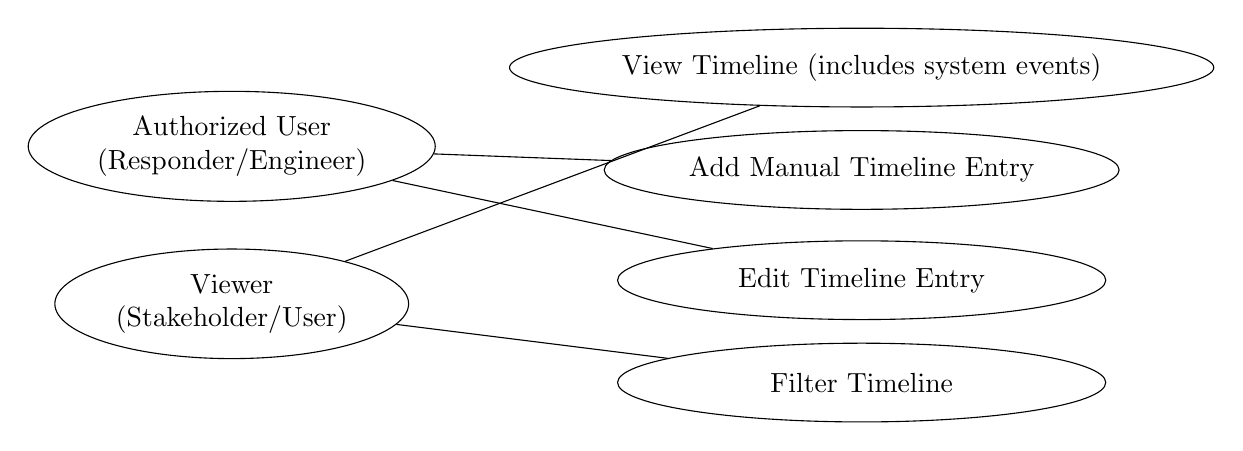
\begin{tikzpicture}[
  actor/.style={draw, ellipse, minimum width=3.0cm, minimum height=1.0cm, align=center},
  usecase/.style={draw, ellipse, minimum width=6.2cm, minimum height=1.0cm, align=center}
]

  \node[actor] (userA) at (-6,1) {Authorized User\\(Responder/Engineer)};
  \node[actor] (viewer) at (-6,-1) {Viewer\\(Stakeholder/User)};

  % Renamed UC-TL-1 label to be diagram-friendly (actor-driven) while still covering system events.
  \node[usecase] (uc1) at (2,2) {View Timeline (includes system events)};
  \node[usecase] (uc2) at (2,0.7) {Add Manual Timeline Entry};
  \node[usecase] (uc3) at (2,-0.7) {Edit Timeline Entry};
  \node[usecase] (uc4) at (2,-2) {Filter Timeline};

  \draw (userA) -- (uc2);
  \draw (userA) -- (uc3);
  \draw (viewer) -- (uc1);
  \draw (viewer) -- (uc4);

\end{tikzpicture}
}
\end{center}

\section{Conceptual Class Diagram (Timeline Domain Model)}
\textit{Note: Conceptual classes only. No methods, access modifiers, or data types.}

\begin{center}
\begin{tikzpicture}[
  class/.style={
    rectangle,
    draw,
    text width=5.2cm,
    align=left,
    minimum height=1.2cm
  }
]

\node[class] (incident) {\textbf{Incident}\\\hline
incidentId\\
title\\
severity\\
state
};

\node[class, right=6.2cm of incident] (event) {\textbf{TimelineEvent}\\\hline
eventId\\
timestamp\\
eventType\\
description
};

\node[class, below=3.2cm of incident] (user) {\textbf{User}\\\hline
userId\\
name\\
role
};

\node[class, below=3.2cm of event] (rev) {\textbf{Revision}\\\hline
revisionId\\
editedAt\\
previousDescription
};

\draw[->] (incident) -- node[above]{contains} node[below]{\small 1 \hspace{1.5cm} 0..*} (event);
\draw[->] (user) -- node[above]{creates} node[below]{\small 1 \hspace{1.5cm} 0..*} (event);
\draw[->] (event) -- node[right]{has} node[left]{\small 1 \hspace{0.6cm} 0..*} (rev);

\end{tikzpicture}
\end{center}

\end{document}